\documentclass[preview]{standalone}
\usepackage{tikz}
\usetikzlibrary{calc}
\usepackage{xcolor}
\definecolor{tordion}{RGB}{0,0,255}
\definecolor{agraviton}{RGB}{255,0,0}
\definecolor{sgraviton}{RGB}{0,255,0}
\begin{document}
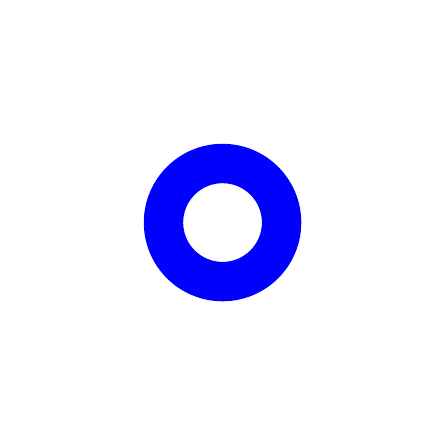
\begin{tikzpicture}[node distance = 1.4cm, auto]
\clip (225:3.5) rectangle (45:3.5);
\coordinate (gauge0) at (45:0);
\fill[tordion,even odd rule] (gauge0) circle (1) (gauge0) circle (0.5);
\end{tikzpicture}
\end{document}
